%
\documentclass[%
 reprint,
 amsmath,amssymb,
 aps,
]{revtex4-1}

\usepackage{graphicx}% Include figure files
\usepackage{dcolumn}% Align table columns on decimal point
\usepackage{bm}% bold math


\begin{document}



\title{VIRTUALIZACIÓN Y CONTENEDORES}
\author{Nilson Laura Atencio}
\affiliation{%
 Universidad Privada de Tacna \textbackslash Facultad de Ingenieria \textbackslash Escuela Profesional de Ingenieria de Sistemas
}%

\begin{abstract}
\begin{center}
\textbf{Resumen}
\end{center}

Las tendencias tecnológicas siguen evolucionando y cada día van apareciendo nuevos conceptos que debemos aprender. Hoy en día casi no se puede tener una discusión respecto a Cloud Computing sin llegar al concepto de “Contenedores” (Containers).  Organizaciones de todos los segmentos de negocio hoy quieren entender que son los contenedores, que significan para las aplicaciones en la nube y como pueden usarlos.
Antes de ahondar en el concepto de contenedores, volvamos unos años atrás para recordar el nacimiento de la virtualización. A medida que el hardware se hacía más poderoso nos encontramos con que el software no ocupaba todas las capacidades de la maquina física donde se encontraba siendo ejecutada (en muchos casos ni siquiera una fracción de estos recursos). Dado lo anterior se crearon recursos “virtuales” para simular el hardware base sobre el cual se ejecuta el software, permitiendo que múltiples aplicaciones puedan ser ejecutadas al mismo tiempo, cada una usando una fracción de los recursos del hardware físico disponible. A a esta “simulación” que permite de compartir recursos la denominamos comúnmente “virtualización”.
.\\

\textbf{Palabras clave:}   virtualizacion, contenedores, herramientas, simulacion, procesos, recursos.\\

\begin{center}
\textbf{Abstract}
\end{center}
In this article we will learn concepts, differences and uses of virtualization and containers, this will allow us to choose the most recommendable option for the performance of a system that is being developed or to make changes in it.\\
\textbf{Keywords:}   virtualization, containers, tools, processes, simulation, resources.\\

\end{abstract}



\maketitle

%\tableofcontents

\section {Introducción}\label{sec:1}

Mucha gente, cuando oye hablar de Docker y de lo que se puede hacer con él, lo primero que piensa es en máquinas virtuales. Al fin y al cabo, una máquina virtual es un software que permite aislarse del sistema operativo subyacente y compartirlo entre varias aplicaciones.
Sin embargo las diferencias entre las tecnologías de contenedores como Docker y las máquinas virtuales son enormes, tanto conceptualmente como en la práctica.
En este artículo vamos a repasar brevemente ambas tecnologías para ver cómo trabajan y entender bien sus diferencias. No volverás a tener dudas al respecto 
Como su propio nombre indica, una máquina virtual (o VM a partir de ahora, de sus siglas en inglés: Virtual Machine) es un sistema operativo completo funcionando de manera aislada sobre otro sistema operativo completo.
La tecnología de VMs permite compartir el hardware de modo que lo puedan utilizar varios sistemas operativos al mismo tiempo.
La filosofía de los contenedores es totalmente diferente a la de las VMs. Si bien tratan también de aislar a las aplicaciones y de generar un entorno replicable y estable para que funcionen, en lugar de albergar un sistema operativo completo lo que hacen es compartir los recursos del propio sistema operativo "host" sobre el que se ejecutan.
Docker Engine se encarga de lanzar y gestionar los contenedores con nuestras aplicaciones, pero en lugar de exponer los diferentes recursos de hardware de la máquina de manera discreta (es decir, 1 procesador y "x" GB de RAM... para cada aplicación), lo que hace es compartirlos entre todos los contenedores optimizando su uso y eliminando la necesidad de tener sistemas operativos separados para conseguir el aislamiento.





%-----------------------------------------------------------------
\section{Objetivos}\label{sec:2}
\subsection{General:}
-  Determinar las características diferenciales las máquinas virtuales y los contenedores.
\subsection{Específicos:}
-  Definir los conceptos de maquinas virtuales y contenedores.\\
- Comparar las definiciones.

%-----------------------------------------------------------------
\section {Marco Teórico}\label{sec:3}

\subsection{Máquinas Virtuales}
\par Una máquina virtual es un software que emula un ordenador justo como si fuese uno real. Todo esto sucede en una ventana dentro de tu sistema operativo actual como cualquier otro programa que uses.La idea de este tipo de software es que puedas ejecutar sistemas operativos como si fuesen una aplicación, mientras este cree que está usando el hardware de un ordenador físico común.
 Cada vez que quieras usar este sistema operativo puedes abrir el software de virtualización y encender tu máquina.
\par Cómo funciona:
	\begin{itemize}
		\item Cuando creas una máquina virtual para instalar otro sistema operativo tendrás que asignar todos los recursos que necesitas: cuánto espacio de disco duro, cuánta memoria RAM, cuanta memoria gráfica, decidir en qué lugar se tendrá el disco duro virtual, etc. Todo esto será tomado de los recursos que tengas en tu ordenador. Esto quiere decir que si, por ejemplo, tienes 16GB de RAM y quieres una máquina virtual con 6GB de RAM, puedes hacerlo. Pero, el sistema operativo original solo tendrá disponible 10GB de RAM cuando la máquina virtual esté encendida. Lo mismo pasa con el disco duro. Si le designas 30GB de espacio en disco, ese espacio quedará clausurado y será usado únicamente por la máquina virtual.
	\end{itemize}
\par Tipos de Máquinas Virtuales
	\begin{itemize}
		\item Máquinas virtuales de sistema:
Las máquinas virtuales de sistema, también llamadas máquinas virtuales de hardware, permiten a la máquina física subyacente multiplicarse entre varias máquinas virtuales, cada una ejecutando su propio sistema operativo. A la capa de software que permite la virtualización se la llama monitor de máquina virtual o hypervisor. Un monitor de máquina virtual puede ejecutarse o bien directamente sobre el hardware o bien sobre un sistema operativo ("host operating system").
		\item Máquinas virtuales de proceso:
Una máquina virtual de proceso, a veces llamada "máquina virtual de aplicación", se ejecuta como un proceso normal dentro de un sistema operativo y soporta un solo proceso. La máquina se inicia automáticamente cuando se lanza el proceso que se desea ejecutar y se detiene para cuando éste finaliza. Su objetivo es el de proporcionar un entorno de ejecución independiente de la plataforma de hardware y del sistema operativo, que oculte los detalles de la plataforma subyacente y permita que un programa se ejecute siempre de la misma forma sobre cualquier plataforma.
El ejemplo más conocido actualmente de este tipo de máquina virtual es la máquina virtual de Java. Otra máquina virtual muy conocida es la del entorno .Net de Microsoft que se llama "Common Language Runtime".
	\end{itemize}
\par¿Cuál es la diferencia entre nube y virtualización?
	\begin{itemize}
		\item La virtualización es una tecnología que separa las funciones del hardware, y las nubes dependen de esa separación. Es fácil confundir ambos conceptos, sobre todo porque ambos se refieren a la creación de entornos útiles a partir de recursos abstractos
La forma más fácil de explicar la diferencia es describirla desde la perspectiva estricta de una infraestructura como servicio (IaaS). La base del cloud computing es un sistema operativo estable (como Linux®). Esta es la capa que proporciona a los usuarios la independencia en los entornos públicos, privados e híbridos. Suponiendo que el acceso a Intranet o a Internet ya está establecido, la virtualización es lo que crea las nubes. El software llamado hipervisor se coloca por encima del hardware físico principal y extrae los recursos de la máquina. Estos recursos pueden ser el potencial de procesamiento en bruto, el almacenamiento o las aplicaciones basadas en la nube que contienen todo el código de tiempo de ejecución y los recursos necesarios para implementarlas.
Si ese es todo el proceso, no se trata de cloud computing, sino de virtualización solamente. Los recursos virtuales deben asignarse a grupos centralizados antes llamarlos nubes, y esas nubes deben coordinarse con software de gestión y automatización antes de que se les pueda considerar cloud computing. Las nubes proporcionan las ventajas adicionales del acceso de autoservicio, el aumento automatizado de la infraestructura y los grupos de recursos dinámicos; esos son los beneficios que marcan más claramente la diferencia con la virtualización tradicional.
	\end{itemize}
\par Aplicaciones de máquinas virtuales 
	\begin{itemize}
		\item Hyper-V virtual machine
		\item VMLite Workstation
		\item Red Hat Virtualization virtual machine
		\item Boot Camp – Solo Mac 
                     \item Microsoft Virtual PC
		\item XenServer
		\item Boot Camp – Solo Mac		
		\item kvm virtual machine\cite{campus}
	\end{itemize}
\par ALas máquinas virtuales  en la Nube
	\begin{itemize}
		\item Microsoft Azure.
		\item  Redmond
		\item Amazon
	\end{itemize}
\subsection{Contenedores}
\par Un contenedor de software se puede considerar como una aplicación para el servidor. Estos se encargan de proporcionar a las aplicaciones archivos, variables y biblotecas que sean necesarios para ejecutarse y maximiza su portabilidad.
Para poder instalar una aplicación, el contenedor se carga en el ordenador en un formato portable o imagen (Image) que incluye todos los datos necesarios para su funcionamiento y, en el ordenador, se inicia en un entorno virtual. \cite{know}
Los contenedores permiten que estos equipos de desarrollo alcancen una eficiencia muy alta en la entrega y el despliegue de software, al solucionar muchos de los retos que presenta la virtualización tradicional.
\par Beneficios:
	\begin{itemize}
		\item Ahorro de espacio y consumo. No se tendrá la necesidad de crear maquinas virtuales en las que instalarlas.
		\item Reutilización. Se puede crear tantas instancias como necesitemos, destruirlas y reproducir el entorno inicial.
		\item No "ensucia". No se tendrá que instalar dentro de nuestro equipo con la problemática que ello conlleva en algunos casos.
		\item Compartir. Estas imágenes las podremos distribuir comodamente entre los componentes de nuestro equipo.
		\item Se obtiene mayor modularidad. El desarrollo con contenedores es ideal para un enfoque basado en microservicios para el diseño de aplicaciones.\cite{campus}
	\end{itemize}
\par Ventajas de los contenedores: \\
Los contenedores de aplicaciones “empaquetan” los recursos necesarios para el funcionamiento de una aplicación sin embargo, las mayores ventajas de tales contenedores radican, sobre todo, en la gestión y en la automatización de software basado en contenedores.\cite{know}
\begin{itemize}
		\item Instalación más sencilla: los contenedores de software se inician a partir de imágenes o representaciones portables de un contenedor, incluyendo un programa y todos los componentes requeridos. De esta manera se compensan las diferencias entre sistemas operativos. Su instalación se reduce a la introducción de una línea de comando.
		\item Independiente de la plataforma: las imágenes se pueden transportar cómodamente de un sistema a otro y se caracterizan por una considerable independencia de la plataforma. Lo único que se necesita para iniciar un contenedor desde una imagen es un sistema operativo que soporte contenedores.
		\item Pérdidas por virtualización mínimas: con un Linux y Docker container, la instalación de contenedores requiere alrededor de 100 MB y unos pocos minutos, aunque no es solo esto a lo que se oponen los administradores de sistemas. Mientras que la virtualización de hardware trae consigo una pérdida de rendimiento para el hipervisor y otros sistemas operativos, los contenedores, al prescindir de todo esto, reducen esta pérdida al mínimo.
		\item Aplicaciones aisladas: cada programa funciona independientemente de otros contenedores, de forma que aplicaciones con requerimientos opuestos pueden funcionar en paralelo en el mismo sistema.
		\item Administración y automatización unitarias: debido a que en una plataforma como Docker todos los contenedores son gestionados con las mismas herramientas, es posible automatizar todas las aplicaciones de manera centralizada. Por esto, estas soluciones están indicadas sobre todo para arquitecturas de servidor en las cuales los componentes están distribuidos en varios servidores, de forma que se carga con los pesos de instancias diferentes. En estos ámbitos de aplicación, el Docker container dispone de herramientas con las cuales configurar automatismos. Esto posibilita, por ejemplo, iniciar instancias nuevas de forma automática en momentos puntuales de sobrecarga. \\
\end{itemize}
\par Al final, el uso de los contenedores es muy conveniente, tambien puede traer un nivel bajo de seguridad estariamos dejando de usar sistemas operativos separados. Pues, los contenedores no son tan herméticos como las máquinas virtuales con sistema operativo propio. En consecuencia, aunque los contenedores constituyen una alternativa para la virtualización de hardware, de momento no la pueden sustituir por completo.\\

\subsection{Diferencias}
	\par Algunos comparan los contenedores con una versión más ligera de las máquinas virtuales, sin embargo pretenden resolver problemas totalmente distintos:
 las máquinas virtuales nacieron para resolver un problema de utilización en los servidores y fundamentalmente abstraen el hardware del sistema operativo, creando un entorno aislado para los sistemas operativos y aplicaciones. 
Y los contenedores nacieron para abstraer las aplicaciones del sistema operativo, de esta forma se pretende hacer las aplicaciones más portables.
\begin{center}
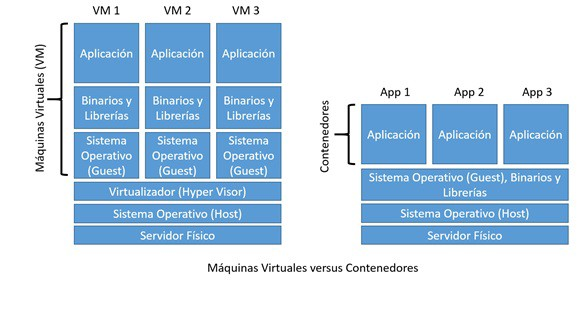
\includegraphics[width=10cm]{./Imagenes/mc}
\end{center}
\par El uso más apropiado de los contenedores o las máquinas virtuales, va a depender del escenario. Algunas de sus diferencias son:\cite{miguel}
\par Las Máquinas virtuales:
	\begin{itemize}
		\item Utilizan una tecnología muy compleja, que se define en el núcleo (kernel) del Sistema Operativo.
		\item Emulan un sistema físico a nivel de hardware: procesador, memoria, unidades de disco, conexiones de red, etc.
		\item Permiten ejecutar varios sistemas simultáneamente.
		\item Estan disponibles a través de proveedores comerciales o soluciones open source, como KVM o Xen.
	\end{itemize}
\par Contenedores:
	\begin{itemize}
		\item Resuelven  los problemas típicos de la virtualización de máquinas.
		\item Pueden ocupar MB en lugar de GB en disco.
		\item No requiere de un hipervisor, se integran en el sistema operativo que los aloja.
		\item El rendimiento del sistema operativo está más optimizado.
		\item El aprovisionamiento de recursos es más rápido.
		\item La disponibilidad de instancias de aplicaciones es más ágil.
		\item Sólo se ejecuta un sistema operativo. \cite{gunnar}
	\end{itemize}

%-----------------------------------------------------------------
\section{Conclusiones}\label{sec:6}


\begin{itemize}
	\item Ambas tecnologías ofrecen ventajas distintas:
La virtualización viene con una plétora de herramientas probadas a lo largo del tiempo, plataformas de gestión y orquestación, sondas virtuales, soluciones de infraestructura virtual hiperconvertidas y mucho más. La portabilidad y la interoperabilidad son las características que destacan frente a los contenedores.
	\item
Los contenedores ofrecen una mayor eficiencia de recursos y agilidad de servicio. Aunque no parezca mucho, abre la puerta a un modelo de microservicios que puede escalar más rápido y de manera más eficiente. Los contenedores de papel se ajustan más a las iniciativas de NFV/SDN y la industria se ha dado cuenta de que 
\end{itemize}


% Bibliografia.
%-----------------------------------------------------------------

\bibliographystyle{plain}
\bibliography{Bibliografia}

\end{document}
